\chapter{Experiments}
\label{chap:experiments}

The proposed pairwise graph convolutional neural networks were evaluated and compared to prior work in both partner specific interface prediction and graph convolution.

\section{Data}

Each model was trained, validated, and tested using complexes from the Docking Benchmark Dataset (DBD) version 5.0~\cite{vreven2015}, a collection of 3D crystalline structures of transient complexes in both the bound and unbound formations. 
DBD is non-redundant in the sense that no two proteins in one complex are in the same Structural Classification of Proteins (SCOP)~\cite{murzin1995} families as two proteins in another complex, respectively.
This ensures the dataset is appropriate for testing since methods that perform better on certain SCOP families than others are not unfairly rewarded or penalized.
Each protein is classified into either \emph{rigid body}, \emph{medium difficulty}, or \emph{difficult}, based on the degree of conformational change of the interfaces.
This is quantified using the root mean squared deviation of the alpha carbons after unbound and bound structures are superimposed on one another. 
Training and validation were performed using the 175 complexes that were present in version 4.0 of DBD, whereas the 55 new complexes added in DBD 5.0 were reserved for testing. 
Training and validation sets were created using a 80\%/20\% partition on the DBD v4.0-only complexes, such that the class proportions in each partition were roughly equivalent.
Hence there were 140 training complexes and 35 validation complexes.
Table \ref{tab:examples} indicates the number of positive and negative examples used from each dataset.

\begin{table}
	\centering
	\begin{tabular}{l l c r r}
		\toprule
		Phase & Data Set & Complexes & Positive examples  & Negative examples \\ 
		\midrule
		\multirow{2}{*}{Model Selection} 
			& Train      & 138       & 12,632 (9.1\%)     & 126,320 (90.9\%) \\
			& Validation & 34        & 3,042 (0.2\%) 		& 1,868,270 (99.8\%) \\
		\midrule
		\multirow{2}{*}{Testing}
			& Train + Validation & 175 & 16,004 (9.1\%) & 160,040 (90.9\%) \\
			& Test       & 55        & 4,871 (0.1\%)      & 4,953,446 (99.9\%) \\ 
		\bottomrule
	\end{tabular}
	\caption{\small Number of complexes and examples (residue pairs) for each phase of experimentation. Negative examples were down sampled to a ratio of 10:1 with positive examples when training, but testing included all examples. During model selection, three complexes were excluded from the training and validation sets due to a software bug and missing features. These complexes were eventually included for the testing phase. \label{tab:dataset_size}}
	\label{tab:examples}
\end{table}

3D structures are contained in Protein Data Bank (PDB) files, which contain atomic coordinates for each amino acid in the complexes.
True interfaces were determined using the bound formations, where two amino acids are assumed to be interacting if they are within 6 \AA{} of each other, in consistent with prior work~\cite{ofran2007, ahmad2011, minhas2014}.
This permits an amino acid residue to interact with multiple partners in the interface.

\subsection{Vertex and Edge Features}
Prediction must be made using the unbound formation of each protein, since the bound formation is not known a priori.
Hence unbound PDB files were used to generate a graph representation of each protein, with vertices indicating residues and edges indicating the relationships between residues.
Features were then computed for each vertex and edge using sequence and structure information from the protein.
Vertex features pertain to the degree of residue conservation, accessible surface area, depth within the protein, and protrusion.
Edge features capture the distance between two residues and their relative orientation as well.
More detail on each feature can be found in Appendix \ref{appendix:features}.

\subsection{Missing Data}
In some cases, features could not be calculated for a residue, resulting in missing values.
For 13 residues, the atomic coordinates of the central alpha carbon were not present in the PDB files, so the Half Sphere Amino Acid Composition, Residue Depth, and $\mathrm{C C_{\alpha} O}$ angle could not be calculated.
Most features rely on third party software to calculate the features from the raw sequence and structure information.
For the proteins with DBD codes 2B42 and 3R9A, features related to the protrusion index could not be calculated for the receptor due to a software fault.
These complexes were omitted during model selection but re-introduced before testing.
Two other complexes, 1NW9 and 1PPE, were also excluded during model selection due to a software bug.
This bug was eventually fixed, so these were also included during testing. 
During model selection, missing values were imputed using the feature mean within a proteins, whereas for testing, the global median (within the training, validation, or test set) was used.
In total there were 138 training and 34 validation complexes during model selection, and there were 175 training and 55 test complexes during testing.
%TODO: find total number of nans?


\section{Experiments}

Experimentation was conducted in two phases: model selection, and testing.
The model selection phase concerned the selection of model \emph{hyper-parameters}, those details which are not explicit model parameters but nevertheless affect the behavior of the network.
For this phase, pairwise graph convolutional networks were repeatedly trained using the training set and evaluated on the validation set.
Once model selection was complete, the final set of model hyper-parameters was used to train and test the most promising hyperparameter configurations and compare them to existing methods.
For this phase, the model was trained on the combined training and validation sets and tested on the test set.


\subsection{Model Selection}

Not only do a network's parameters ($\Theta$) help determine the network's output, but the set of hyper-parameters as well.
Hyper-parameters comprise all model specifications besides the parameters themselves, such as the number and types of layers, number of units/filters in each layers, choice of nonlinear activation function, loss function, and training details.
Hyper-parameters are typically chosen either by some automated process, or by manual exploration.

Automated hyper-parameter selection processes include a randomized search, grid search, or a sequential, model based optimization (SMBO) algorithm such as a Gaussian Process or Tree Structured Parzen Estimator~\cite{bergstra2011}.
The advantage of these approaches is their ability to automatically search a hyper-parameter space without human intervention. 
SMBO approaches are able to estimate the performance "response surface" in hyper-parameter space in order to efficiently find the optimum value.
The disadvantage of these approaches is they sometimes require a large number of iterations in order to converge to optimal parameters, and it may be difficult to incorporate human prior knowledge about the optimal set of hyper-parameters.
Some experiments were performed with SMBO algorithms, but none produced hyper-parameters which outperformed results found by human exploration.
One hindering factor for the automated approaches was the sheer number of parameters being explored, making it difficult to sample the space in an efficient way.
%TODO: report number of hyperparameters tried?
Therefore automated approaches were abandoned in favor of a manual search.

Several hyper-parameters were explored manually by training/validating networks under different settings of the hyper-parameters.
This exploration occurred in a one-hyper-parameter-at-a-time fashion, alleviating the exponential problems encountered with the automated algorithms, but also limiting the ability to explore the interactions between different hyper-parameters.
Following is a list of different hyper-parameters which were explored and the general trends encountered in each.
\begin{itemize}
	\item Number of convolutional layers:
	\item Number of convolution filters:
	\item Receptive field size:
	\item Number of dense layers after merge:
	\item Parameter inizialization: weights and biases
	\item Nonlinear activation function:
	\item 
	\item Loss function:
	\item Update algorithm:
\end{itemize}

The cumulative findings of and intuition gained from the manual model selection procedure informed the final set of experiments which were run in the testing phase of experimentation.

\subsection{Testing}

Final model testing was performed for both sum coupled and product coupled graph convolutions.
For each variant, receptive field sizes of 11 and 21 were tested (the central vertex plus 10 or 20 neighbors, respectively), with one, two three, and four graph convolutional layers. 
In total, 16 hyper-parameter conditions were tested, all of which used the following training scheme:
The number of filters for networks with one convolutional layer was 256, Likewise for two, three, and four convolutional layers the number of filters was (256, 512), (256, 256, 512), and (256, 256, 512, 512) respectively. 
After merging examples, dense layers of 256 and 1 units respectively were applied, with the latter producing the model output.
Loss was computed using weighted cross entropy, a measure of the dissimilarity between two probability distributions. 
Since this is a binary classification problem, the cross entropy for a single example $x$ is defined as: 

\hl{Need to figure out this WEIGHTED cross entropy stuff.}
\begin{equation}
\mathbb{H}(x, y) = - y 
\label{eq:weighted_ce}
\end{equation}

) where the network output for an example $x$ is interpreted as a logit value, $f(x)=log(p/{1-p})$, where $p$ is the predicted probability that the example is a positive.

Most weights were initialized by drawing from a uniform distribution between $-\tau_0$ and $\tau_0$, where $\tau_0=\frac{1}{\sqrt{n_{in}}}$ and $n_{in}$ is the number of inputs to a connected layer. (is this right?) (is this really He initialization?).
All Biases were initialized to zero.
Stochastic gradient descent was performed with a learning rate of 0.1, mini-batch size of 128 pairs, for 80 epochs. 
Dropout with probability $p=0.5$ was performed during training.

The networks were implemented in TensorFlow~\cite{abadi2015} v1.0.1 and trained using a single NVIDIA GTX 980 or GTX TITAN X GPU.
Training time varied from 9 to 46 minutes, depending on network size, GPU card, and computer resource availability.
Figure \ref{fig:train_times} shows that training time increases roughly linearly in the number of convolutional layers.

\begin{figure}
	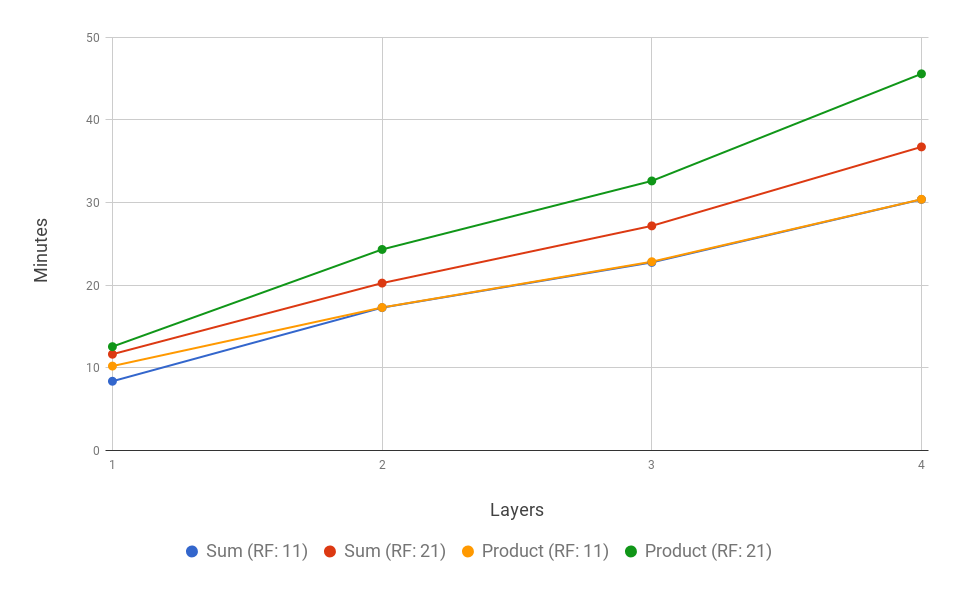
\includegraphics[width=0.8\textwidth]{training_times.png}
	\caption{Training time for pairwise graph convolution neural network, during testing. Times are shown for sum and product coupled convolutions, receptive fields of size 11 and 21, and 1-4 convolutional layers. Training time scales roughly linearly with the number of layers, with different slopes likely due to differences in machine resources and GPU.
	\label{fig:train_times}}
\end{figure}


\section{results}
\subsection{metrics}

Compared against diffusion convolutions and PAIRpred.

\begin{table}
\begin{center}
	\begin{tabular}{lccccc}
		\toprule
		\multirow{2}{*}{Method} &
		Receptive Field & \multicolumn{4}{c}{Layers Before Merge} \\
		& Size & 1 & {2} & {3} & {4} \\
		\midrule
		No Convolution & N/A & \textbf{0.815} & 0.812 & 0.800 & 0.811  \\\cline{1-6}
		\multirow{2}{*}{GCN-SC} & 11 & 0.868 & 0.889 & 0.882 & 0.884 \\
		& 21 & 0.875 & \textbf{0.903} & 0.880 & 0.890 \\\cline{1-6}
		\multirow{2}{*}{GCN-PC} & 11 & 0.856 & 0.869 & 0.885 & 0.868 \\
		& 21 & 0.863 & 0.876 & 0.896 & \textbf{0.899} \\
		\bottomrule
	\end{tabular}
	\caption{\small Median area under the receiver operating characteristic curve (AUC) across all complexes in the test set for two variants of Graph Convolutional Networks (GCN), \textit{sum-coupled} (SC) and \textit{product-coupled} (PC). Results are shown for two different sizes of receptive field, 11 and 21, for different numbers of convolutional layers before the pairwise merge operation. Bold faced values indicate best performance for each method.}
	\label{tab:med_auc}
\end{center}
\end{table}

\begin{table}
	\begin{center}
		\begin{tabular}{lccccc}
			\toprule
			\multirow{2}{*}{Method} &
			Receptive Field & \multicolumn{4}{c}{Layers Before Merge} \\
			& Size & 1 & {2} & {3} & {4} \\
			\midrule
			No Convolution & N/A & \textbf{48} & 55 & 53 & 66 \\\cline{1-6}
			\multirow{2}{*}{GCN-SC} & 11 & 32 & 28 & 70 & 86 \\
			& 21 & \textbf{26} & 37 & 56 & 63 \\\cline{1-6}
			\multirow{2}{*}{GCN-PC} & 11 & 30 & 46 & 26 & 51 \\
			& 21 & 26 & \textbf{25} & 36 & 37 \\
			\bottomrule
		\end{tabular}
		\caption{\small Median rank of the first positive prediction (RFPP) across all complexes in the test set for two variants of Graph Convolutional Networks (GCN), \textit{sum-coupled} (SC) and \textit{product-coupled} (PC). Results are shown for two different sizes of receptive field, 11 and 21, for different numbers of convolutional layers before the pairwise merge operation. Bold faced values indicate best performance for each method (lower is better).}
		\label{tab:med_rfpp}
	\end{center}
\end{table}

\begin{figure}
	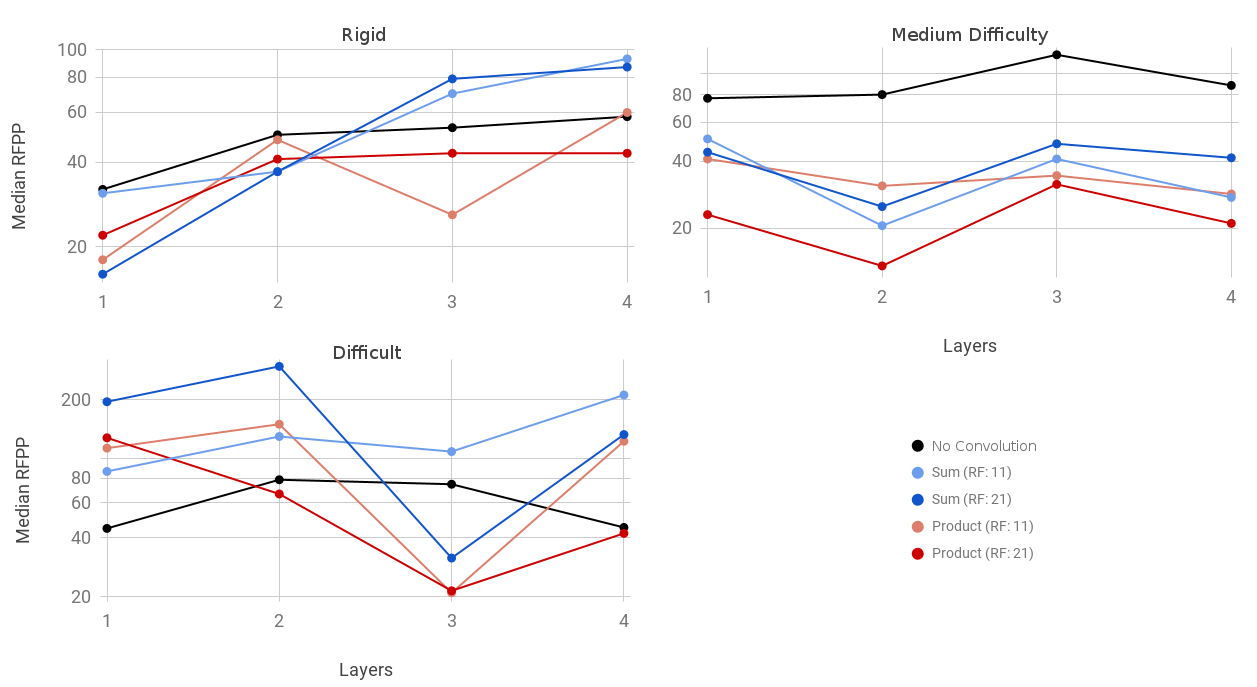
\includegraphics[width=\textwidth]{med_rfpp.png}
	\caption{Median rank of the first positive prediction (RFPP) across all complexes in the test set, separated by complex class. Vertical axes are log scaled. Sum and product coupling are shown for two receptive field sizes each (11 and 21), as well as no convolution, for 1-4 pre-merge layers. Lower RFPP is better. Best performance on rigid complexes is achieved with just one layer in for all networks. Generally, as difficulty increases, so does the number of layers needed to achieve best results.
		\label{fig:med_rfpp}}
\end{figure}

\begin{figure}
	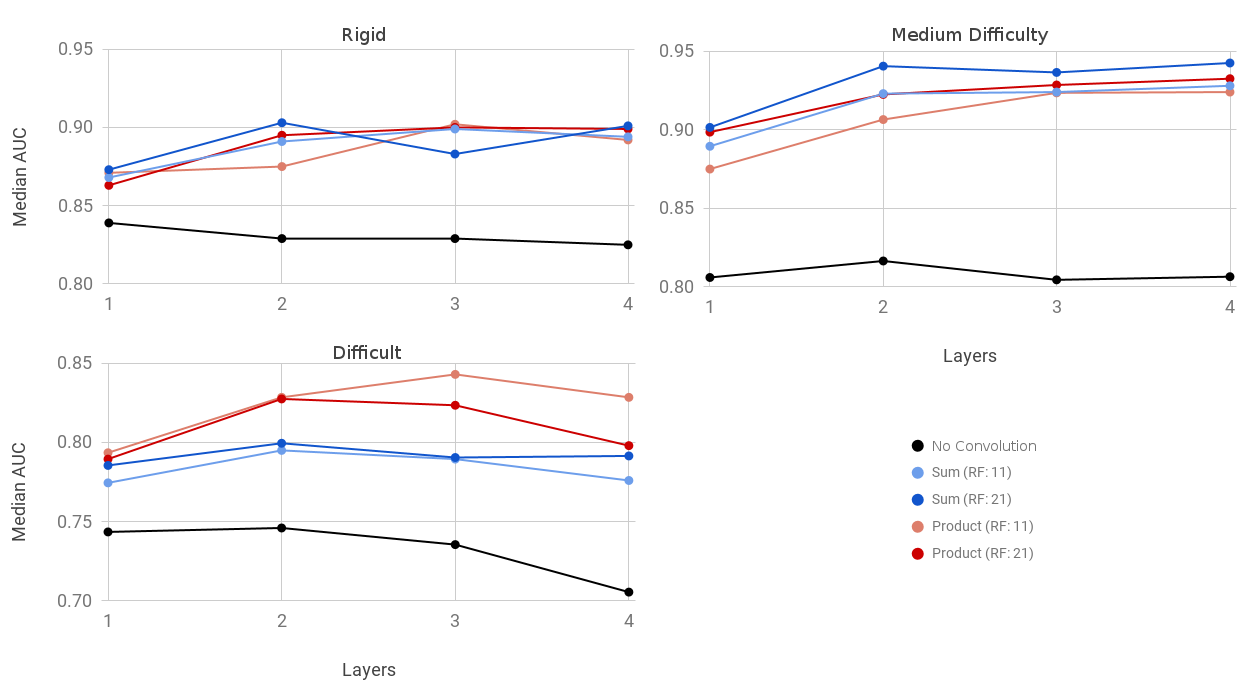
\includegraphics[width=\textwidth]{med_auc.png}
	\caption{Median area under the receiver operating characteristic curve (AUC) across all complexes in the test set, separated by complex class. Sum and product coupling are shown for two receptive field sizes each (11 and 21), as well as no convolution, for 1-4 pre-merge layers. For rigid and medium difficulty complexes, performance does not significantly increase beyond two layers. For difficult complexes, product coupling is actually hindered beyond 3 layers. No convolution is hindered beyond 2 layers. 
		\label{fig:med_rfpp}}
\end{figure}

